% !TeX spellcheck = en_GB
% !TeX program = pdflatex
\documentclass[10pt,a4paper]{article}
\usepackage[british]{babel}
\usepackage{cvstyle}

\begin{document}

\begin{sidebar}
{\Large Petr \textsc{Šimčák}}\par\vspace*{0.4ex}
{\small Tech Lead \& Software Developer}\par\vspace*{1.8ex}

\centering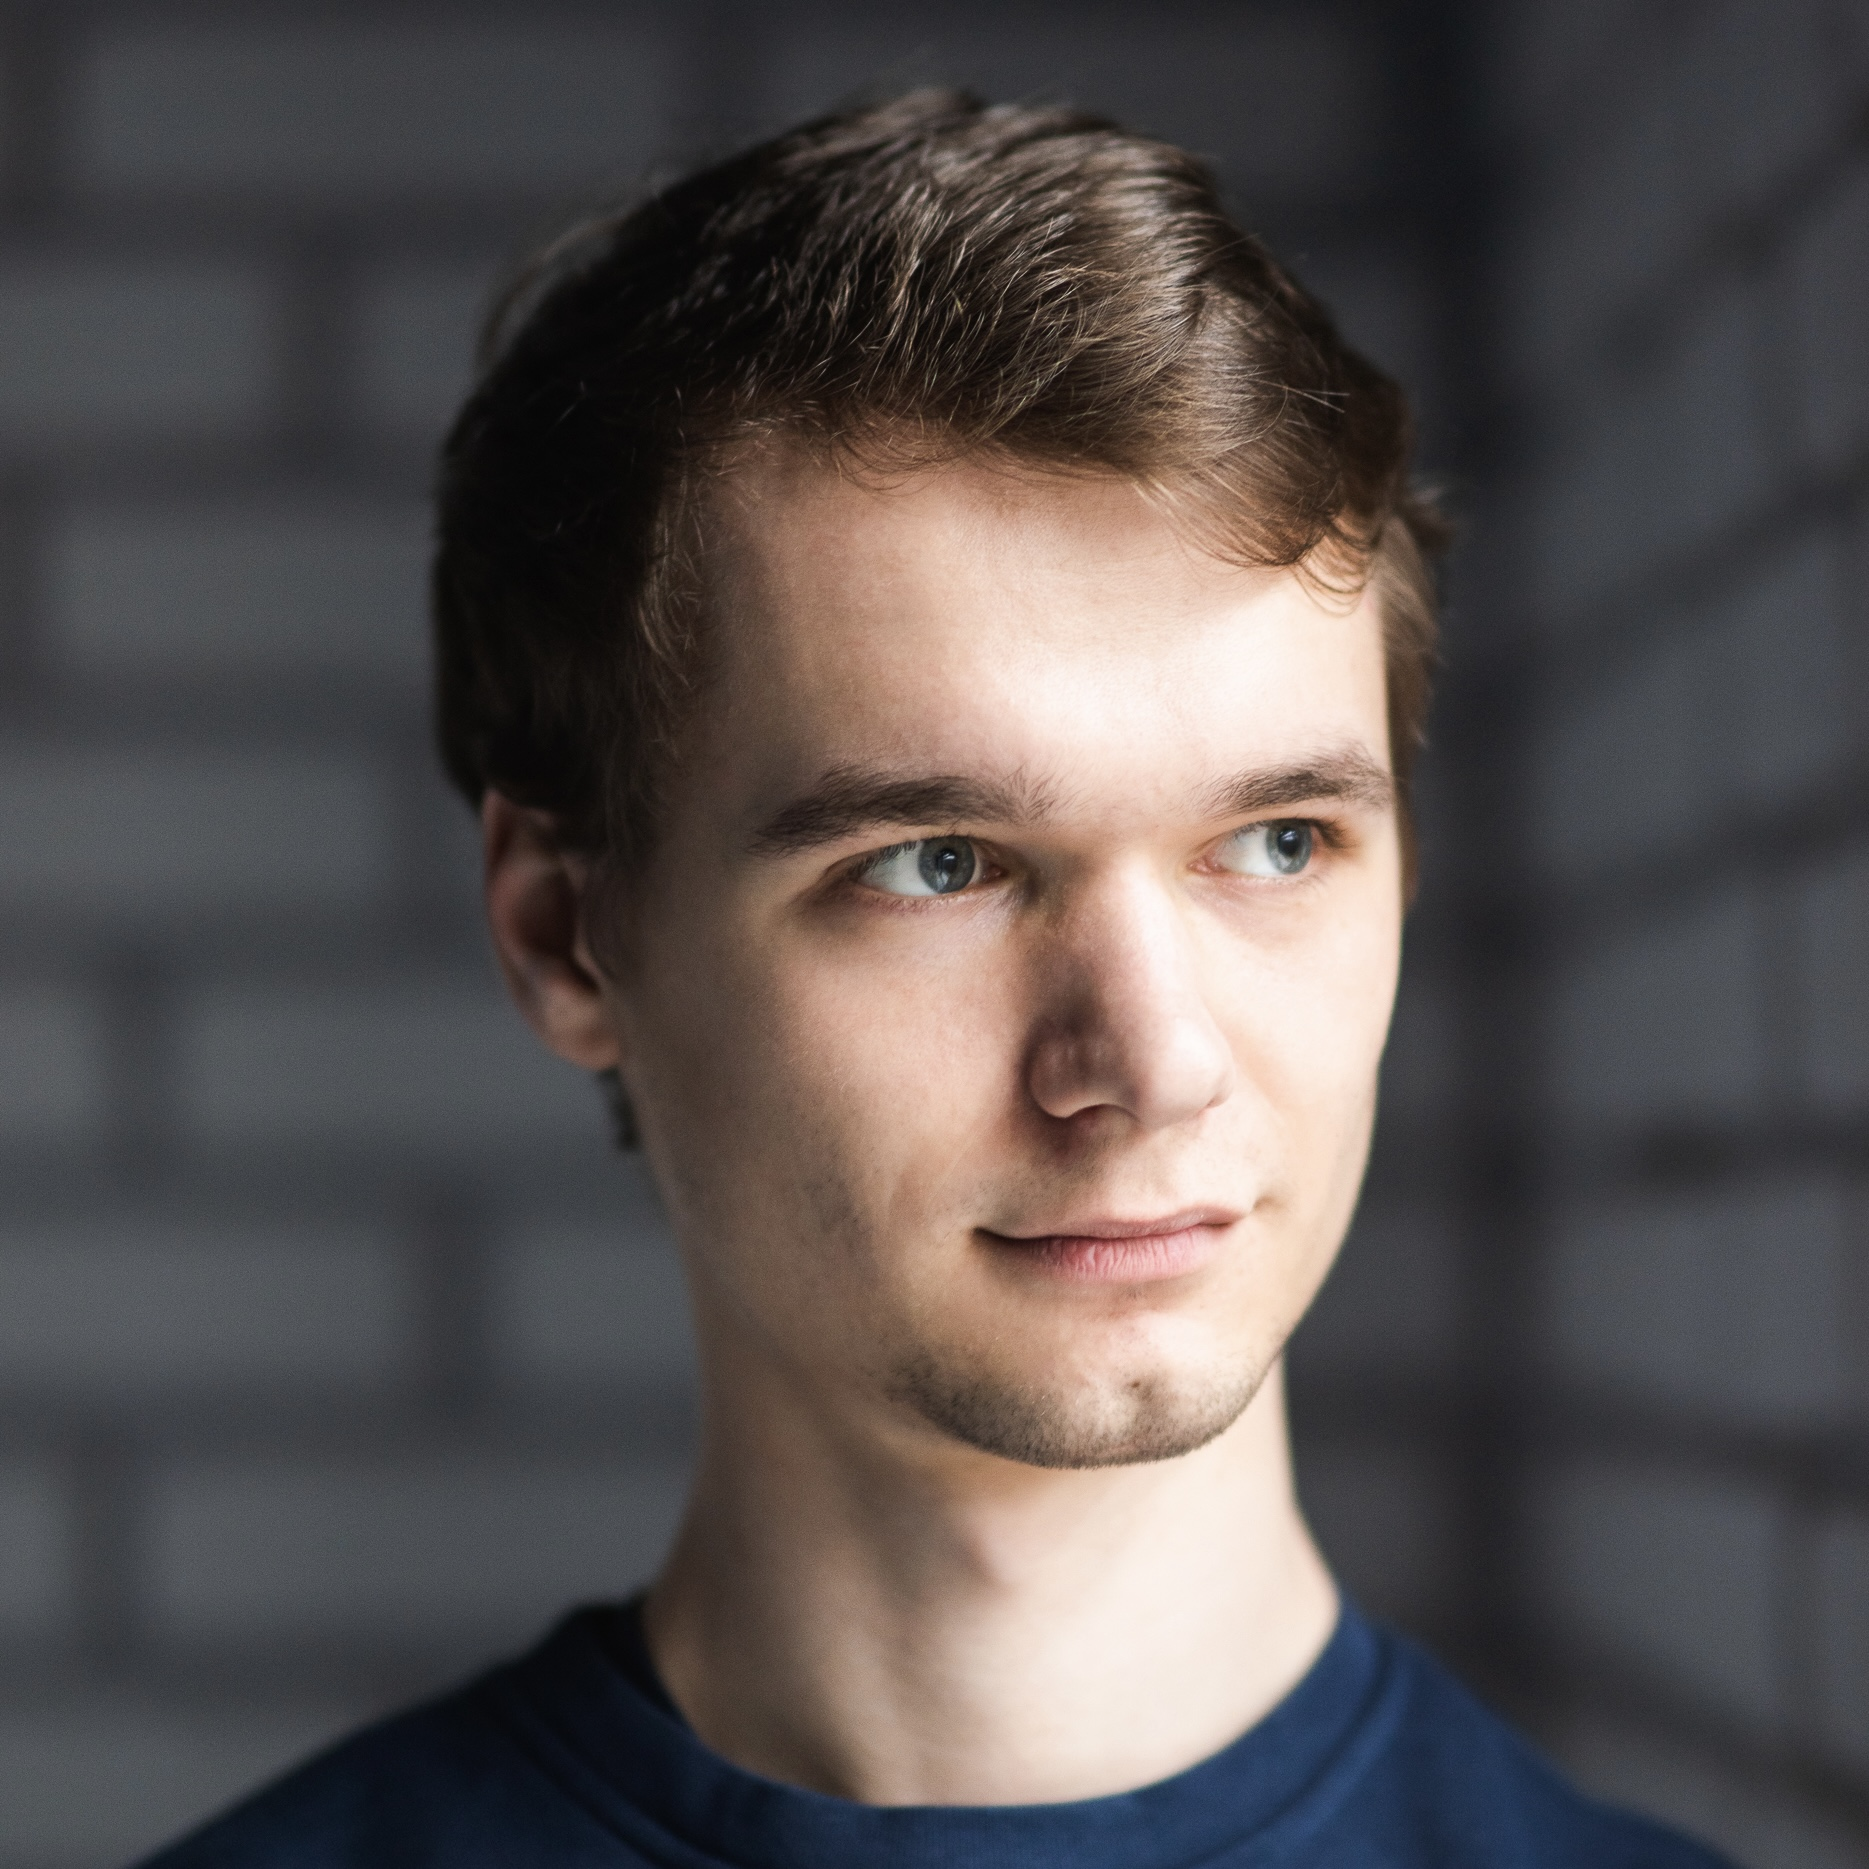
\includegraphics[width=0.8\textwidth]{me.jpg}\par
\raggedright

\sidehead{About me}
Tech Lead at AI Camp and software developer who came to technology from theatre and film.
I am interested in how AI changes the way people work and organisations operate.
I look for the balance between speed and quality -- efficiency that does not sacrifice the result.
I combine technical thinking with communication and presentation skills, and I enjoy most turning ideas into things that work.

\sidehead{Contact}
{\small
\contact{\faEnvelope}{\href{mailto:peta.simcak@gmail.com}{peta.simcak@gmail.com}}
\contact{\faPhone}{+420\,601\,381\,619}
\contact{\faMapMarker*}{Prague, Czech Republic}
\contact{\faGlobe}{\href{https://simcak.github.io}{simcak.github.io}}
\makebox[1.5em][l]{\faLinkedin}\href{https://www.linkedin.com/in/petr-simcak}{linkedin.com/in/petr-simcak}\par}

\sidehead{Skills}
{\small
\begin{itemize}
\item Practical use of LLMs and AI tools, AI training for companies
\item C, C++, Python, JavaScript, Shell, SQL, MATLAB
\item Git, Docker, Linux, Nginx, LaTeX
\item Backend, frontend, systems and network programming
\item Signal processing and analysis
\end{itemize}}

\sidehead{Languages}
{\small
Czech (native) \\[0.4ex]
English (C1) \\[0.4ex]
German (B1)\par}

\sidehead{Awards \& more}
{\small
\begin{itemize}
\item 1st place in the Education Platform category, Greenhack (2026)
\item 3rd place, Škoda Hackathon (2025)
\item 2nd place, Škoda Hackathon (2024)
\item Best Young Actor, Zlín Film Festival (2014)
\end{itemize}}
\end{sidebar}%
\begin{maincolumn}

\mainhead{Work experience}

\cventry{Tech Lead}{AI Camp}{2026 -- present}{%
\begin{itemize}
\item Tutoring and supporting clients from large companies in using LLMs and other AI technologies efficiently and creatively.
\item Responsible for maintaining and developing the AI Camp curriculum and internal tools.
\end{itemize}}

\cventry{Software Developer}{Moneco, Broker Consulting group}{2026}{%
Designed and built OK-Form, a voting and prioritisation app for an investment committee that replaced Google Forms. It runs with no server, database or monthly fees: a static site on GitHub Pages, ballots collected by e-mail and results processed automatically into CSV and Excel with GitHub Actions and Python. \href{https://github.com/custom-alg/OK-Form}{GitHub}}

\cventry{Hitchhiker}{42 Prague}{2026 -- present}{%
Representing the school and its values at events, supporting new students and taking responsibility for a fair study process for others.}

\cventry{3D Printer Maintenance}{BUT Brno, 42 Prague}{2022 -- present}{%
Assembled a 3D printer at BUT and later ran, maintained and supported the 3D~printers at 42~Prague.}

\cventry{Film Actor}{Czech, German and US productions}{2013 -- 2021}{%
Roles in films and TV series in several languages; lead role in \textit{To See the Sea} (2014). Long-term collaboration in demanding productions, working under pressure and discipline. \href{https://www.imdb.com/name/nm5791331/}{IMDb}}

\cventry{Theatre Actor}{Brno City Theatre}{2009 -- 2015}{%
Seven productions from the age of eight, including one of the lead roles in the musical Mary Poppins. \href{https://www.mdb.cz/cs/lide/petr-simcak}{Theatre profile}}

\mainhead{Selected projects}

\cventry{Škoda Hackathon -- 3rd place}{Team Lead / Backend}{2025}{%
Led team B3R Brigade, which built a working application for internal talent search and mobility at Škoda Auto during the hackathon, covering both the employee and the HR perspective (FastAPI, React, Docker, SQLite).}

\cventry{ft\_transcendence}{FastAPI, React, Docker, PostgreSQL}{2026}{%
Team-based full-stack web application: an audiobook marketplace with audio streaming. \href{https://github.com/simcak/Core/tree/main/16_FT_TRANSCENDENCE}{GitHub}}

\cventry{ft\_irc}{C++98, sockets, poll}{2026}{%
IRC server for hundreds of users, developed in a team of three; my main contribution was the server structure and IRC commands. \href{https://github.com/simcak/Core/tree/main/14_IRC}{GitHub}}

\cventry{Cub3D}{C, MLX42}{2025}{%
Simplified raycasting engine in the style of Wolfenstein~3D. \href{https://github.com/simcak/Core/tree/main/11_CUB3D}{GitHub}}

\mainhead{Education}

\cventry{42 Prague}{software engineering}{2023 -- 2026}{%
Project-based curriculum built on peer learning (2024--2025 at 42~Heilbronn). Projects include minishell and Inception: Unix processes, shell logic, containerisation and deployment. \href{https://github.com/simcak/Core}{GitHub}}

\cventry{Brno University of Technology}{BSc, Sport Technology}{2020 -- 2025}{%
Thesis \textit{Heart Rate Estimation from PPG Signals} (Python): comparison of heart-rate estimation methods for physiological signals and automatic signal-quality assessment. \href{https://github.com/simcak/bakalarka}{GitHub}}

\end{maincolumn}

\end{document}
